\section{Tree-To-Text Transformation with SDMs}
\begin{enumerate}
\item[$\blacktriangleright$] DictionaryTreeGrammar
  (Fig.~\ref{fig:moca-DictionaryTreeGrammar})    
  %\usepackage{graphics} is needed for \includegraphics
\begin{figure}[!htbp]
\begin{center}
 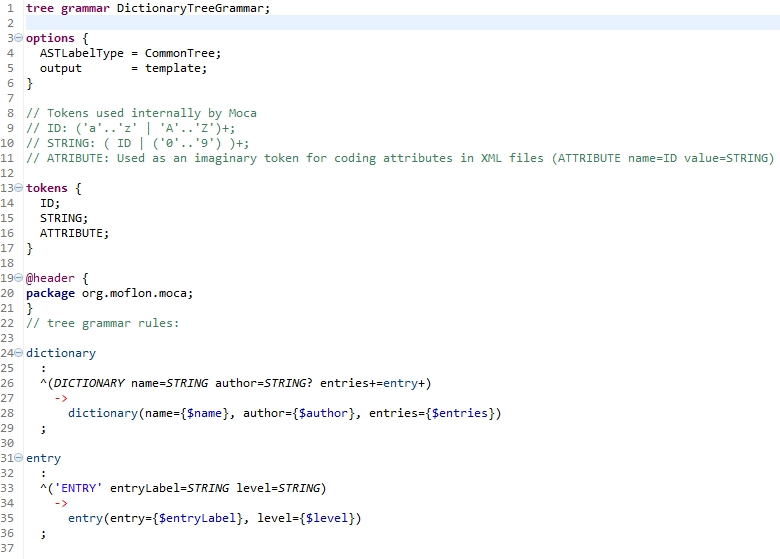
\includegraphics[width=\textwidth]{pics/moca/4ModelToMocaTree/DictionaryTreeGrammar}
  \caption{Tree Grammar for the dictionary DSL} 
  \label{fig:moca-DictionaryTreeGrammar}
\end{center}
\end{figure} 

\item[$\blacktriangleright$] DictionaryUnparserAdapter
  (Fig.~\ref{fig:moca-DictionaryUnparserAdapter})    
  %\usepackage{graphics} is needed for \includegraphics
\begin{figure}[!htbp]
\begin{center}
 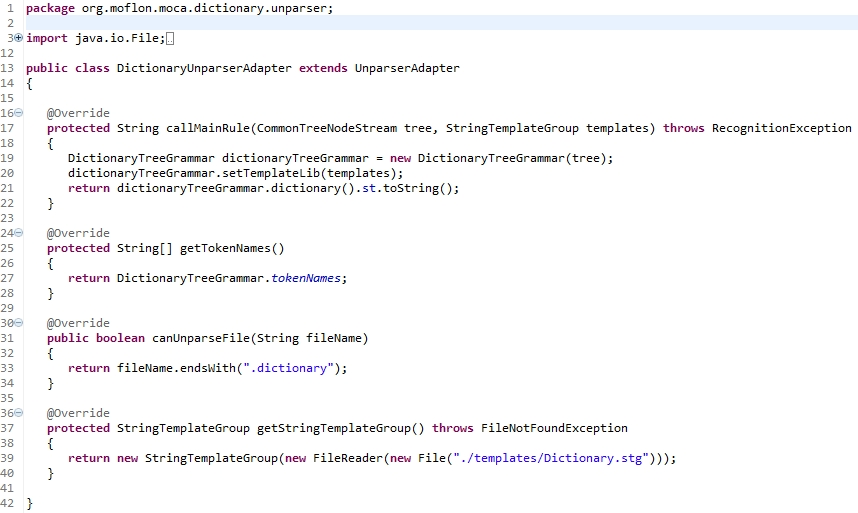
\includegraphics[width=\textwidth]{pics/moca/4ModelToMocaTree/DictionaryUnparserAdapter}
  \caption{Unparser Adapter} 
  \label{fig:moca-DictionaryUnparserAdapter}
\end{center}
\end{figure} 

\item[$\blacktriangleright$] Templates
  (Fig.~\ref{fig:moca-DictionaryTemplates})    
  %\usepackage{graphics} is needed for \includegraphics
\begin{figure}[!htbp]
\begin{center}
 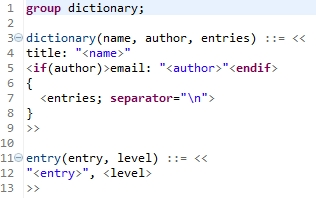
\includegraphics[width=0.6\textwidth]{pics/moca/4ModelToMocaTree/DictionaryTemplates}
  \caption{Templates for the Dictionary DSL} 
  \label{fig:moca-DictionaryTemplates}
\end{center}
\end{figure} 

\item[$\blacktriangleright$] As a final step, open \texttt{MocaMain.java}
(Fig.~\ref{fig:moca-8-MocaMain}) and add the following lines:
\begin{verbatim}
// Perform tree-to-text (using initial tree)
codeAdapter.unparse("instances", out);
\end{verbatim}
\end{enumerate}